\pdfoutput=1

\documentclass{l4proj}

%
% put any packages here
%
\usepackage{float}
\usepackage{enumitem}
\usepackage{longtable}
\usepackage{listings}

\begin{document}
\title{On The Scalability of ROS}
\author{Isaac Jordan}
\date{\today}
\maketitle

\begin{abstract}
Robots, distributed systems, and middleware.
\end{abstract}

\educationalconsent
%
%NOTE: if you include the educationalconsent (above) and your project is graded an A then
%      it may be entered in the CS Hall of Fame
%
\tableofcontents
%==============================================================================

\chapter{Introduction}
\pagenumbering{arabic}

\section{Context}

Robotics is the field of creating physical systems to automate tasks. As a concept, automation dates back hundreds of years - however the idea of replicating biological systems seen in nature (for example, humans) was not first seen until the 20th century. Robotics was mainly considered a theoretical or fictitious fantasy, however the main discussers of the concept (such as Isaac Asimov) assumed technological capability would inevitably reach the level where robotics would either be inseperable from society, or be banned due to it's impact.

In the 19th century the beginnings of robotics could be seen in the creation of vehicles which could be remotely operated using electric signals. By the early 20th century, wireless radio guidance systems were advanced enough that remotely operated aircraft could be demonstrated in 1917 (by Archibald Low [citation needed]).

Technology advanced so rapidly during the 20th century that by the 1970s the Soviet Union could explore the surface of the moon using a remotely operated vehicle robot.

However, these uses of robotics displayed no `intelligent behaviour' on behalf of the robotic system. Beginning in the 1980s, the growing field of Artificial Intelligence (A.I.) was revived and began creating systems which could intelligently answer domain-specific questions - called expert systems.

Robotics is a fast-progressing field which has seen major advances the past decades. From obvious examples such as Amazon's item pickers, to more integrated applications such as autonomous cars - the scale of robotics is increasing.

\section{Aims and Objectives}

If I had an aim it would go here.

\section{Achievements}

If I had achieved anything it would go here.



%\vspace{-7mm}
%\begin{figure}
%\centering
%\includegraphics[height=9.2cm,width=13.2cm]{uroboros.pdf}
%\vspace{-30mm}
%\caption{An alternative hierarchy of the algorithms.}
%\label{uroborus}
%\end{figure}

\chapter{Background}

\section{Robotics}

Robots are the future. (Why robots are important)

Robotics is the field concerning autonomous computer systems, usually involving physical interaction with it's environment. Robotics lies at the intersection between computing science, eletrical and mechanical engineering. Robotics has been common in popular culture since the 1940s, however the physical realisation of these systems did not begin to be practical until the 2000s when increases in computing power, sensor accuracy, research investment, and software algorithms allowed for useful robotics systems to be created.

Today's robotic systems generally consist of many small autonomous systems working together to form a coherent whole. For example, a particular sensor (say a camera) may be constantly recording data and storing it in some buffer (erasing the oldest when full). This subsystem does not depend on any others to complete it's task (recording the envionrment), but other subsystems may rely on it's output (such as a computer vision package which needs video frame inputs).

Robotics is part of a field called cyber-physical systems (CPS) that concerns computer systems that interface with the physical world. These can include Internet Of Things (IOT) networks which can (for example) be used to control things around the household, such as light switches, central heating systems, and hoovering. This is distinct from robotics as CPS generally embody a `think globally, act locally' approach (such as using data from many sources to improve the CPS' performance in each), compared to robotics which utilises a more `think locally, act locally' strategy - meaning that each instance of a robot generally makes it's own decisions, and acts upon them solely.

\section{Multi-Robot Systems}

Multi-robot systems are specific instances of mult-agent systems. They represent a joint problem space between robotics, artificial intelligence, and distributed systems. Multi-robot systems as a formal concept is a recent development with a IEEE technical committee only being formed in 2014\cite{MultiRobotSystemsIEEECommittee}.

Multi-robot systems can consist of many intelligent agents (each of which may be comprised of many small autonomous systems) working to solve a task that any one system may not be able to solve alone. One such example is a warehouse management system.

In a warehouse, millions of items can be spread throughout miles of shelving and the requirement is that a random subset of items (those that have been bought) must arrive at a specific point (the delivery pick-up point) at a specific time (when the van is there). This task previously could be solved by having human pickers wander the isles searching for items - however given recent increases in the size of online shopping this is no longer feasible. Now, online retailers are using thousands of individual robots to intelligently move the shelving around and bring the correct items to stationary human pickers. This system requires the coordination of the individual robots, but they must all act independently in order to efficiently keep pace with the items ordered.

\section{Scalability in Robotics}

When creating multi-robot systems, scalability becomes an important concern. At what level does a system architect choose to switch from small highly-powered robot systems to a larger number of simpler robot systems. Several factors to consider include the processing power of each robot, the communication framework required to organise them, the cost of each robot, and the suitability of the problem to a multi-robot system.

Swarm robotics is the extreme approach of creating many very simple robots which individually could not solve tasks or survive environments - however when they work together as a form of society they can work efficiently.

\section{Robotic Middleware}

Robot designers want to work at a high level. Sensors are low level. (Why is middleware needed, whats available)

Robotic middleware is a software infrastructure that is intended to provide convenient abstraction and communication paradigms for facilitating this multi-subsystem approach. In general, a robotics middleware would provide interfaces for defining each subsystem, and defning how each subsystem communicates with others.

Robots consist of many individual sensors, for example a camera that can record 720p RGB video at 30fps, a LIDAR range sensor that can measure distances of up to 30m at a frequency of 1-500Hz, a tri-axis gyroscope and accelerometer capable of measuring up to 16g of force with a measurement frequency of 40Hz. These devices use a range of sophisticated technologies to measure and analyse the physical world, each recording a different data format at a different data rate. These sensor modules are all independently designed, resulting in a wide array of different software and hardware interfaces - meaning that each robot system that wishes to use these sensors must create the software to communicate with these sensors, consume their data, and then write the robotic software that makes use of it. This results in a wide variety of implementations for manipulating the same data on each sensor, increasing the likelihood of implementation mistakes, misunderstandings, and wasting researchers' time.

Software called middleware is the solution to this problem. A middleware provides a common interface design so that no matter what hardware is creating the data, the results are distributed in a consistent manner. This means that hardware manufacturers (or users) need only implement one software system for each sensor that can them be distributed and reused amongst all users of that sensor, as long as those users are using that middleware. This means that creators of systems utilising that middleware have easy access to the data created by a particular sensor as they know the software the create will be able to easily consume the sensor's data stream.

Another benefit of middleware is that this communication interface can be reused within the robotic system for communicating between distinct modules within the system. For example, a researcher may create a computer vision module that processes a video stream and returns a data stream containing a description of the objects in the video stream at each frame. When utilising a middleware, the researcher can make the result of their computer vision module available in a similar fashion to the sensor's video stream - meaning that higher level software can utilise the results as if there was an `object-detecting hardware sensor'. These levels of abstractions make software much more maintainable, and reusable.

There are a wide variety of robotic middlewares in use currently. Many employ a free (libre) approach to software by making the source code available online, whereas others are created for commercial licensing using propriatary source.

\subsection{An Overview}

\begin{center}
	\setitemize[0]{leftmargin=*}
	\begin{longtable}{| l | l | l | l | l |}
		\hline
		\textbf{Name} & \textbf{Objective} & \textbf{Support} & \textbf{Capabilities} & \textbf{Supported Languages} \\ \hline

		\begin{minipage}[t]{0.1\columnwidth}%
		ROS (Robot Operating System) %
		\end{minipage} &
		\begin{minipage}[t]{0.25\columnwidth}%
			\begin{itemize}
				\item The goal of ROS is not to be a framework with the most features. Instead, the primary goal of ROS is to support code reuse in robotics research and development
				\item Keep libraries ROS-agnostic
				\item Easy to test
				\item Scalable; appropriate for large runtime systems, and large development processes
			\end{itemize} %
		\end{minipage} &
		\begin{minipage}[t]{0.1\columnwidth}%
			Large, active open source development %
		\end{minipage} &
		\begin{minipage}[t]{0.25\columnwidth}%
			\begin{itemize}
				\item Can be used in conjunction with other robot frameworks
				\item Distributed framework of processes allows for executables to be individually designed, and loosely coupled at runtime
				\item Encourages collaboration by easy package sharing
				\item Not a realtime framework, although can work with realtime code
			\end{itemize} %
		\end{minipage} &
		\begin{minipage}[t]{0.2\columnwidth}%
			Python, C++, and Lisp \newline

			Experimental: Java, and Lua %
		\end{minipage} \\
		\hline

		\begin{minipage}[t]{0.1\columnwidth}%
		MOOS (Mission Oriented Operating Suite) %
		\end{minipage} &
		\begin{minipage}[t]{0.25\columnwidth}%
			\begin{itemize}
				\item Designed to facilitate research in the mobile robotic domain
				\item Constitute a resilient, distributed and coordinated suite of software suitable for in-the-field deployment of sub-sea and land research robots
				\item Process communcation should be utterly robust and tolerant of repeated stop/start cycling of any process
			\end{itemize} %
		\end{minipage} &
		\begin{minipage}[t]{0.1\columnwidth}%
			Not widely used (judging by GitHub stars at least) \newline

			Development is stagnating (no GitHub commits since 26th May 2016), core not updated since 11th May 2016 %
		\end{minipage} &
		\begin{minipage}[t]{0.25\columnwidth}%
			\begin{itemize}
				\item Platform independent, inter-process communication API
				\item Sensor management
				\item Navigation
				\item Concurrent mission task execution
				\item Vehicle safety management
				\item Mission logging and replay
				\item No P2P communication (client/server only)
			\end{itemize} %
		\end{minipage} &
		\begin{minipage}[t]{0.2\columnwidth}%
			C++ (appears to have Python bindings) %
		\end{minipage} \\
		\hline

		\begin{minipage}[t]{0.1\columnwidth}%
		YARP (Yet Another Robot Platform) %
		\end{minipage} &
		\begin{minipage}[t]{0.25\columnwidth}%
			\begin{itemize}
				\item Supports collection of programs communicating P2P
				\item Extensible family of connection types (tcp, udp, multicast, local, MPI, XML, RPC, …)
				\item Flexible interfacing with hardware devices
				\item Goal to increase the longevity of robot software projects
			\end{itemize} %
		\end{minipage} &
		\begin{minipage}[t]{0.1\columnwidth}%
			Active, open source effort %
		\end{minipage} &
		\begin{minipage}[t]{0.25\columnwidth}%
			\begin{itemize}
				\item Data carrier method seems more flexible than ROS
				\item General network set up seems similar to ROS. Many processes across one or more machines communicating P2P using Observer design pattern. \cite{YARP_it_notes}
				\item Supports more operating systems than ROS
			\end{itemize} %
		\end{minipage} &
		\begin{minipage}[t]{0.2\columnwidth}%
			SWIG (binding auto-generator) %
		\end{minipage} \\
		\hline

		\begin{minipage}[t]{0.1\columnwidth}%
		Orocos (Open RObot Control Software) %
		\end{minipage} &
		\begin{minipage}[t]{0.25\columnwidth}%
			\begin{itemize}
				\item Component based system design
				\item Multi vendor (doesn’t aim to solve every problem, but facilitate use of many projects)
				\item Focus (aims to be the best free software framework for realtime control of robots and machine tools, nothing more, nothing less)
			\end{itemize} %
		\end{minipage} &
		\begin{minipage}[t]{0.1\columnwidth}%
			Non-active. Still in use, but by very few people (judging by forum activity, and documentation errors (listed source host has gone down). No `news' since 2013. %
		\end{minipage} &
		\begin{minipage}[t]{0.25\columnwidth}%
			\begin{itemize}
				\item Provides toolchain to create realtime robotics applications using modular, run-time configurable software components
				\item Provides Kinematics and Dynamics Library for modelling and computation of kinematic chains, their motion specification, and interpolation (basically controlling things like robot arms)
			\end{itemize} %
		\end{minipage} &
		\begin{minipage}[t]{0.2\columnwidth}%
			C++ %
		\end{minipage} \\
		\hline

		\begin{minipage}[t]{0.1\columnwidth}%
		CARMEN (Carnegie Mellon Robot Navigation Toolkit) %
		\end{minipage} &
		\begin{minipage}[t]{0.25\columnwidth}%
			\begin{itemize}
				\item Open source collection of software for mobile robot control
				\item Modular software to provide basic navigation functionalities, such as base and sensor control, logging, obstacle avoidance, localization, path planning, and mapping
			\end{itemize} %
		\end{minipage} &
		\begin{minipage}[t]{0.1\columnwidth}%
			Discontinued, no new releases since 2008. %
		\end{minipage} &
		\begin{minipage}[t]{0.25\columnwidth}%
			\begin{itemize}
				\item Uses inter-process communication platform IPC
				\item Centralised parameter server
				\item Only supports a limited number of specific mobile robot bases.
			\end{itemize} %
		\end{minipage} &
		\begin{minipage}[t]{0.2\columnwidth}%
			C and Java %
		\end{minipage} \\
		\hline

		\begin{minipage}[t]{0.1\columnwidth}%
		Orca %
		\end{minipage} &
		\begin{minipage}[t]{0.25\columnwidth}%
			\begin{itemize}
				\item Open source framework for developing component-based robotic systems
				\item Goal to enable software reuse by defining commonly used interfaces
			\end{itemize} %
		\end{minipage} &
		\begin{minipage}[t]{0.1\columnwidth}%
			Discontinued, no new releases since 2009 %
		\end{minipage} &
		\begin{minipage}[t]{0.25\columnwidth}%
			\begin{itemize}
				\item Provides some interfaces and implementations of commonly used components
				\item No particular distributed network things
				\item Seems to use client/server architecture
			\end{itemize} %
		\end{minipage} &
		\begin{minipage}[t]{0.2\columnwidth}%
			C++, examples in Java, Python, and PHP. \newline

			Interfaces can be compiled to C++, Java, Python, PHP, C\#, Visual Basic, Ruby, and Obj C. %
		\end{minipage} \\
		\hline

		\begin{minipage}[t]{0.1\columnwidth}%
		Microsoft Robotics Developer Studio (v4) %
		\end{minipage} &
		\begin{minipage}[t]{0.25\columnwidth}%
			\begin{itemize}
				\item Goal to make creating robotics applications very accessible
				\item Supports visual programming (drag and drop components)
				\item Supports simple “Hello Robot” to complex applications in mutli-robot scenarios
			\end{itemize} %
		\end{minipage} &
		\begin{minipage}[t]{0.1\columnwidth}%
			No release since 2012 %
		\end{minipage} &
		\begin{minipage}[t]{0.25\columnwidth}%
			\begin{itemize}
				\item REST-style, services oriented runtime
				\item Supports centralised, and decentralised communcation
			\end{itemize} %
		\end{minipage} &
		\begin{minipage}[t]{0.2\columnwidth}%
			C\#, and Microsoft Visual Programming Language (VPL) %
		\end{minipage} \\
		\hline

		\begin{minipage}[t]{0.1\columnwidth}%
		OpenRTM-aist %
		\end{minipage} &
		\begin{minipage}[t]{0.25\columnwidth}%
			\begin{itemize}
				\item Open source platform to develop component oriented robotic systems.
			\end{itemize} %
		\end{minipage} &
		\begin{minipage}[t]{0.1\columnwidth}%
			Seems moderately active (last release May 2016). Moderately active community (more popular in Japan) %
		\end{minipage} &
		\begin{minipage}[t]{0.25\columnwidth}%
			\begin{itemize}
				\item Supports communication based on Publisher/Subscriber model
				\item Has a number of tools for robot system development
			\end{itemize} %
		\end{minipage} &
		\begin{minipage}[t]{0.2\columnwidth}%
			C++, Python, Java %
		\end{minipage} \\
		\hline

		\begin{minipage}[t]{0.1\columnwidth}%
		Player %
		\end{minipage} &
		\begin{minipage}[t]{0.25\columnwidth}%
			\begin{itemize}
				\item Provides a clean and simple interface to the robot's sensors and actuators over the IP network
			\end{itemize} %
		\end{minipage} &
		\begin{minipage}[t]{0.1\columnwidth}%
			Discontinued \newline

			No commits since May 2016 \newline

			No releases since 2012 %
		\end{minipage} &
		\begin{minipage}[t]{0.25\columnwidth}%
			\begin{itemize}
				\item Supports multiple concurrent connections between devices
				\item Supports flexible network structure (including P2P)
			\end{itemize} %
		\end{minipage} &
		\begin{minipage}[t]{0.2\columnwidth}%
			Clients in C++, Tcl, Java, and Python %
		\end{minipage} \\
		\hline

		\begin{minipage}[t]{0.1\columnwidth}%
		ROS2 %
		\end{minipage} &
		\begin{minipage}[t]{0.25\columnwidth}%
			\begin{itemize}
				\item Target new use cases, such as multi-robot systems (providing a standard approach), embedded systems, real-time systems, non-ideal networks, and production environments \cite{why_ros2}
				\item Recreate ROS using existing new tech (such as Redis, WebSockets, DDS)
				\item Overhaul of API (create consistent API without > 7 years of backward compatibility)
			\end{itemize} %
		\end{minipage} &
		\begin{minipage}[t]{0.1\columnwidth}%
			Pre-release, but active daily development. Unstable but good future prospects given popularity of ROS1 %
		\end{minipage} &
		\begin{minipage}[t]{0.25\columnwidth}%
			\begin{itemize}
				\item Improved communication resilience on poor networks utilising DDS \cite{kozik-ros2evaluation} \cite{Maruyama:2016:EPR:2968478.2968502}
				\item Communication overhead of DDS shown to be non-trivial for local connection. For remote, overhead is trivial but throughput depends on DDS library used \cite{Maruyama:2016:EPR:2968478.2968502}
			\end{itemize} %
		\end{minipage} &
		\begin{minipage}[t]{0.2\columnwidth}%
			C99, C++11, Python3 \newline

			Speculative: JavaScript %
		\end{minipage} \\
		\hline

		\begin{minipage}[t]{0.1\columnwidth}%
		OpenRDK %
		\end{minipage} &
		\begin{minipage}[t]{0.25\columnwidth}%
			\begin{itemize}
				\item Modular framework for distributed robotic systems
				\item Communication achieved by a central `repository' into which individual agents publish variables (and can store queues)
				\item Uses URL-like addressing scheme
				\item Focuses on mobile robots \cite{4651213}
			\end{itemize} %
		\end{minipage} &
		\begin{minipage}[t]{0.1\columnwidth}%
			Open source, no news since 2010, created for a single research group %
		\end{minipage} &
		\begin{minipage}[t]{0.25\columnwidth}%
			\begin{itemize}
				\item Created with an eye on the competition (not a copy of another framework)
				\item Has been used in multiple environments (single rescue robotic system, assistive robots) \cite{4651213}
				\item Has useful tools such as a graphical tool for remote inspection and management of modules, and also modules for logging and replaying \cite{4651213}
				\item No real-time support \cite{OpenRDKIntro}
			\end{itemize} %
		\end{minipage} &
		\begin{minipage}[t]{0.2\columnwidth}%
			C++ %
		\end{minipage} \\
		\hline

		\begin{minipage}[t]{0.1\columnwidth}%
		Miro %
		\end{minipage} &
		\begin{minipage}[t]{0.25\columnwidth}%
			\begin{itemize}
				\item Builds upon other-widely used middlewares (ACE, TAO CORBA, Qt) to provide object-oriented abstractions \cite{1044362}
				\item Split in to 3 layers: Device, Service, and Framework
				\item Communication achieved using CORBA client/server
			\end{itemize} %
		\end{minipage} &
		\begin{minipage}[t]{0.1\columnwidth}%
			Last release was 2014 %
		\end{minipage} &
		\begin{minipage}[t]{0.25\columnwidth}%
			\begin{itemize}
				\item Provides same capabilities as CORBA (type-safe and network-transparent interfaces) \cite{1044362}
				\item Demonstrated capabilities in multirobot environment
				\item Does not have true OS independence (all robots used Linux), but shown that this can be ported to Solaris in 1 day
			\end{itemize} %
		\end{minipage} &
		\begin{minipage}[t]{0.2\columnwidth}%
			Any that have CORBA implementations %
		\end{minipage} \\
		\hline

		\begin{minipage}[t]{0.1\columnwidth}%
		Xenomai %
		\end{minipage} &
		\begin{minipage}[t]{0.25\columnwidth}%
			\begin{itemize}
				\item Real-time development framework (can be used to create any kind of real-time interface)
				\item Important goals are extensibility, portability, and maintainability
				\item Uses a dual-kernel approach to hard realtime \cite{choi2009real}
			\end{itemize} %
		\end{minipage} &
		\begin{minipage}[t]{0.1\columnwidth}%
			Sustained, active, open source development \cite{XenomaiGitRepos} %
		\end{minipage} &
		\begin{minipage}[t]{0.25\columnwidth}%
			\begin{itemize}
				\item Poor availability of detailed documentation and a lack of technical support \cite{koh2013real}
				\item Runs on top of an OS (most commonly the Linux kernel)
				\item Shown to be suitable for 100\% hard real-time applications \cite{brown2010fast}
				\item No communication abstractions
			\end{itemize} %
		\end{minipage} &
		\begin{minipage}[t]{0.2\columnwidth}%
			Preferred C \cite{XenomaiTutorial} \newline

			Possible: C++ %
		\end{minipage} \\
		\hline

		\begin{minipage}[t]{0.1\columnwidth}%
		CORBA (Common Object Request Broker Architecture) %
		\end{minipage} &
		\begin{minipage}[t]{0.25\columnwidth}%
			\begin{itemize}
				\item Software-based communications interface through which objects are located and accessed
				\item OO abstractions utilising request-response in the library (via the Object Request Broker)
				\item Uses Interface Definition Language (IDL) to define object interfaces
			\end{itemize} %
		\end{minipage} &
		\begin{minipage}[t]{0.1\columnwidth}%
			Active, open source and proprietary implementations %
		\end{minipage} &
		\begin{minipage}[t]{0.25\columnwidth}%
			\begin{itemize}
				\item Criticised for poor implementations of the standard
				\item Good language and OS independence
				\item `Freedom from technologies', meaning that (for example) C++ code can talk to Fortran legacy code and Java database code (and each can be changed independently without having to update the other code bases)
				\item Strong typing of messages, reducing human error
				\item Small overhead to adding to system (but dependent on implementation)
				\item Has real-time implementations of related standard (realtime CORBA)
			\end{itemize} %
		\end{minipage} &
		\begin{minipage}[t]{0.2\columnwidth}%
			Ada, C++, Java, COBOL, Lisp, Python, Ruby, Smalltalk \newline

			Non-standard mappings exist for C\#, Erlang, Perl, Tcl, Visual Basic %
		\end{minipage} \\
		\hline

		\begin{minipage}[t]{0.1\columnwidth}%
		Urbi %
		\end{minipage} &
		\begin{minipage}[t]{0.25\columnwidth}%
			\begin{itemize}
				\item Urbiscript aims to provide a programming experience tailored towards robotics (parallel, event-based, functional, OO, client/server, distributed)
				\item Consists of defining modules called `UObject's which are shells around regular components
				\item These UObjects are then naturally supported by urbiscript which allows easier communication and orchestration
			\end{itemize} %
		\end{minipage} &
		\begin{minipage}[t]{0.1\columnwidth}%
			Doesn’t appear to be widely used, but is open source with many commits %
		\end{minipage} &
		\begin{minipage}[t]{0.25\columnwidth}%
			\begin{itemize}
				\item Interoperable with CORBA, RT-Middleware, openHRP (among others), thus URBI can act as a central platform to integrate other technologies
				\item Brings many useful abstractions over other middlewares such as Player/Stage, Microsoft Robotics Studio, RT-Middleware, and CORBA.
				\item Can move UObject’s after compile-time
			\end{itemize} %
		\end{minipage} &
		\begin{minipage}[t]{0.2\columnwidth}%
			C++, Java \newline

			Custom “urbiscript” scripting language for orchestration %
		\end{minipage} \\
		\hline

	\end{longtable}
\end{center}

\subsection{Communication}

\subsection{Computation}

\subsection{Configuration}

\subsection{Coordination}


\section{ROS (Robot Operating System)}

ROS is what I'll be testing out. (What is it)

\section{Configuration of Robots}

The robots used in this project are 9 identical robot cars with front-wheel steering. (What is their set up)


\chapter{Experimental Analysis}

\section{Experiment 1}

The first experiment was designed to analyse the transfer time of messages between two machines at varying message frequencies. This would highlight whether there was some limit as to how often ROS could send and receive messages on it's topics.

\subsection{Configuration}

These two machines were Raspberry Pi 3 Model Bs connected via ethernet to an Asus router.

The messages were sent and received using ROS Kinetic, running on the Raspbian OS.

The experimental setup was that one Raspberry Pi would run a ROS master node, another Raspberry Pi runs a sender program that notes down the message-sent time, and sends it to a 3rd Raspberry Pi which merely echoes the message back to the sender. Upon receiving the message, the sender/receiver notes the current time, and writes `message X which was sent at Y, was received at Z' to a text file. The resulting Round Trip Time (RTT) for each message would therefore be the difference between the message-sent time and the message-received time.

The expected result of the experiment was that message latency (RTT) would be the same across all lower frequencies, until some bottleneck was reached that would then cause message latencies to exponentially increase due to congestion.

Code had been written prior to execute this experiment, so initially this was used \ref{Exp1InitCode}. However, this gave results that were contrary to the hypothesis. An increase in message frequency resulted in a reduction in message latency. A number of messages on higher frequencies were also dropped, and never received. As this was the opposite of the hypothesis, the first step was to critique the experiment code.

This review highlighted two major issues, the first was the echoing machine had a delay similar to the sender when the experiment design mandated that the echoer always respond as fast as it can. The second issue was the the maximum message queue size in ROS (how many messages can be buffered at once to compensate for a slow subscriber) was set equal to the message frequency of that run.

These issues were resolved by removing the code that executed the delay in the echoer, and by setting the maximum queue size to be equal to 1000 in every experiment (the number of messages expected to be sent).

The experiment was then repeated using this code, and the results from these runs agreed with the hypothesis.

\section{Experiment 2}

Experiment 2 was an investigation in to whether the performance of ROS messages was affected by previous messages sent on the system. This was tested by comparing the performance of ROS messages of 5 consecutive message passing runs vs 5 message passing runs with system reboots between runs. This was repeated at 1KHz, 4KHz, 7KHz, and 10Khz frequencies for two reasons. The first was to investigate whether areas in which we observed consistent performance before would exhibit any difference between reboot and no reboot. Secondly, it would give further insight in to where the exact barrier between `good, consistent performance' and `poor, erratic performance' is.

Rebooting the systems involved has the opportunity to affect performance by stopping any background processes, interrupting slow processing messages from previous runs, and resetting any message caches and buffers in memory.

The result of the experiment was hypothesised to demonstrate no significant difference between rebooting and not-rebooting at any message frequency.

\begin{figure}[h]
\centering
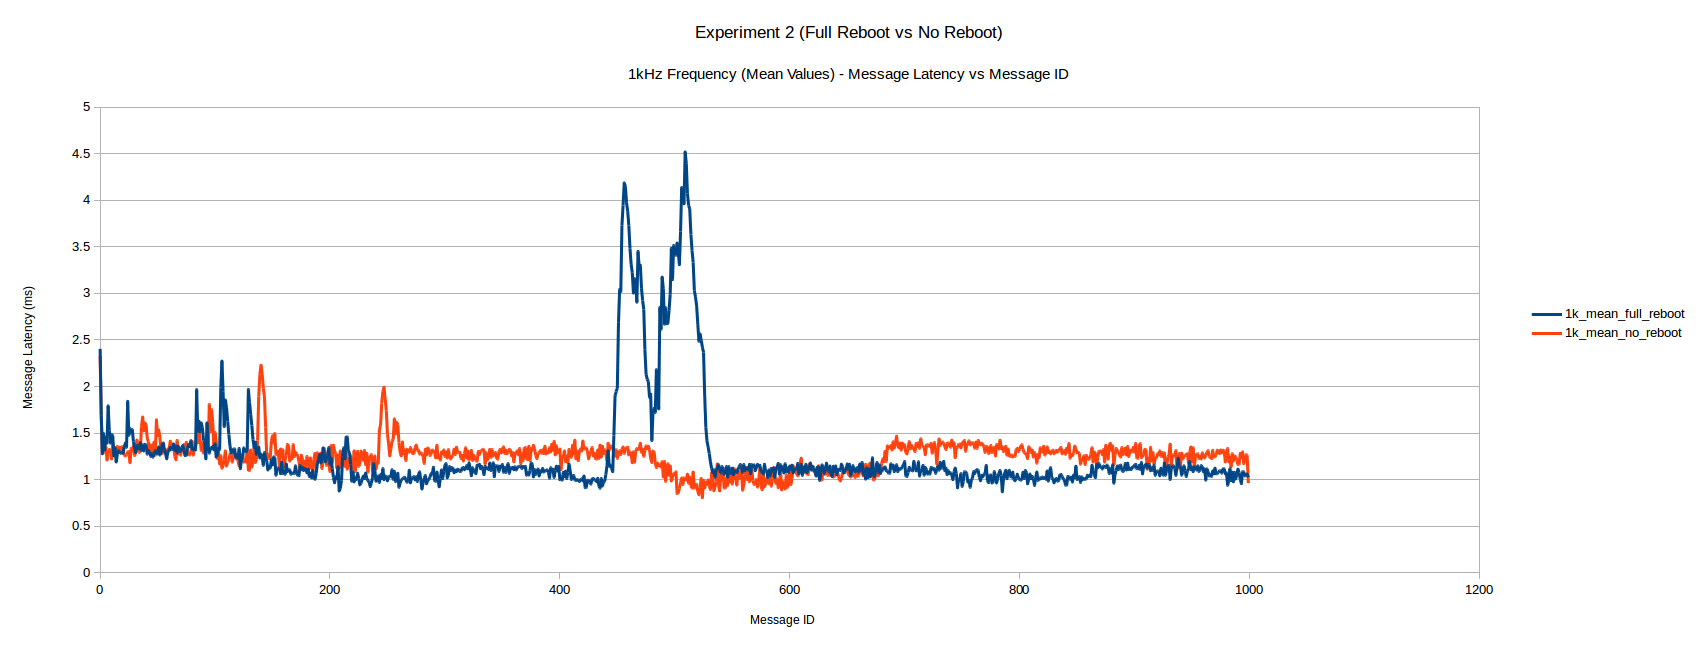
\includegraphics[width=\textwidth]{images/1khz-mean.png}
\caption{Experiment 2 - Mean Message Latency 1KHz Message Frequency}
\label{exp2-1khz-mean}
\end{figure}

Figure \ref{exp2-1khz-mean} demonstrates that for relatively low message frequencies the mean message latency was consistently 1 - 1.5ms (the peak around message 500 in the full reboot data was due to 1 erroneous run at that data point). Figure \ref{exp2-4khz-mean} is characteristic of the higher frequency runs - the no reboot runs generally gave equal or better performance compared to the full reboot runs. See Appendix \ref{exp2-appendix-results} for other mean graphs, and individual run graphs.

\begin{figure}[h]
\centering
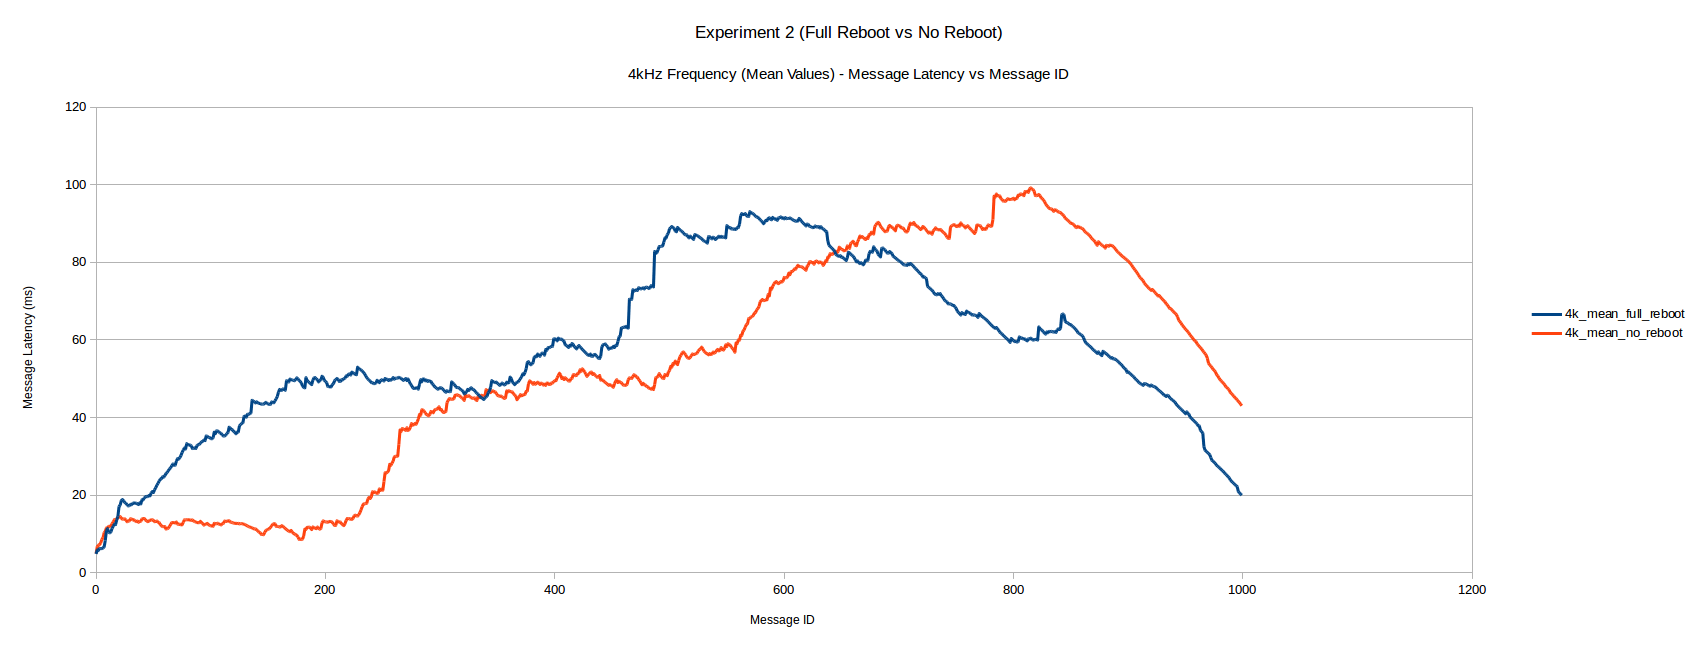
\includegraphics[width=\textwidth]{images/4khz-mean.png}
\caption{Experiment 2 - Mean Message Latency 4KHz Message Frequency}
\label{exp2-4khz-mean}
\end{figure}

%%%%%%%%%%%%%%%%
%              %
%  APPENDICES  %
%              %
%%%%%%%%%%%%%%%%
\begin{appendices}

\chapter{Experiment 2 Other Graphs}
\label{exp2-appendix-results}

\begin{figure}
\centering
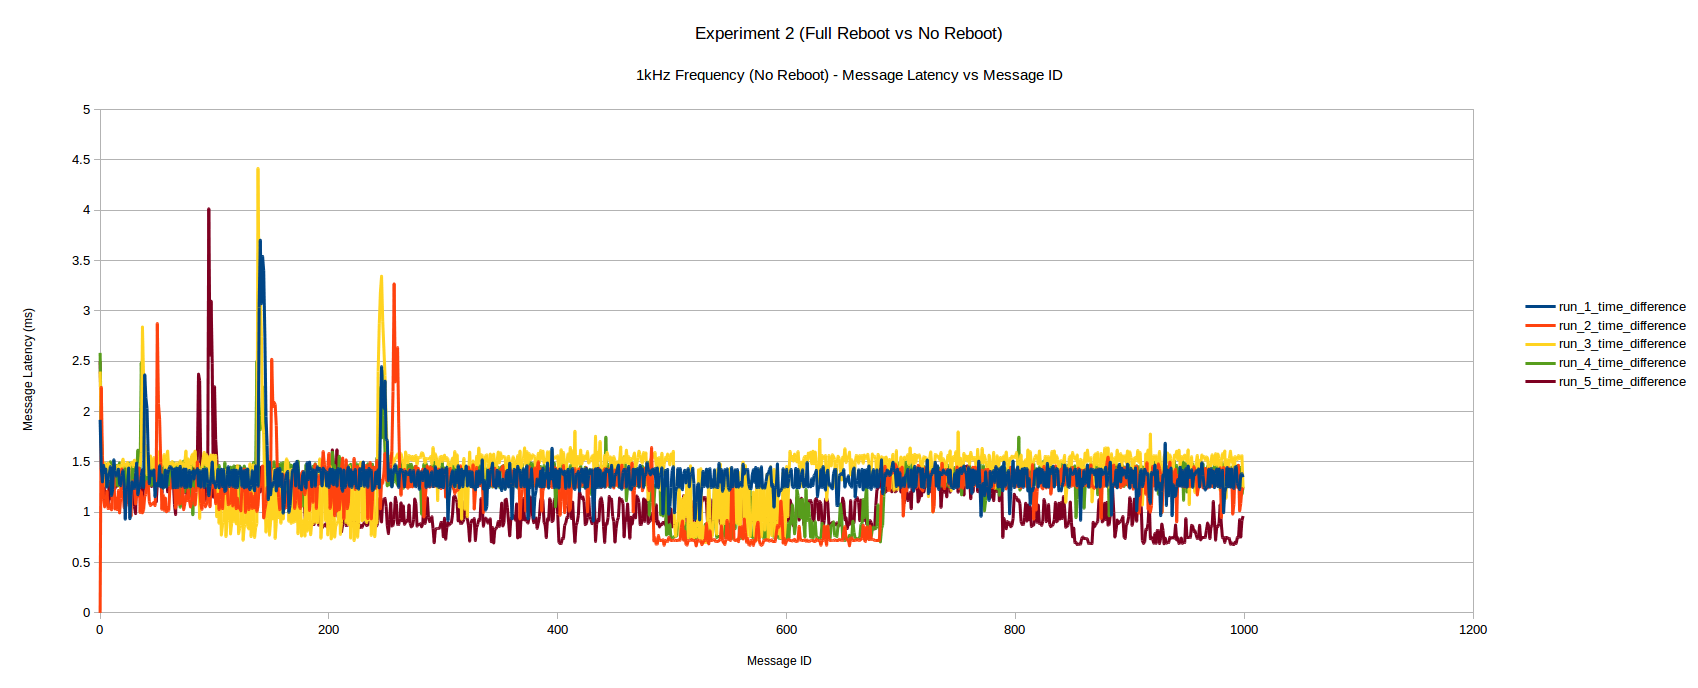
\includegraphics[width=\textwidth]{images/no-reboot-1khz.png}
\caption{Experiment 2 - No Reboot 1KHz Message Frequency}
\label{exp2-noreboot-1khz}
\end{figure}

\begin{figure}
\centering
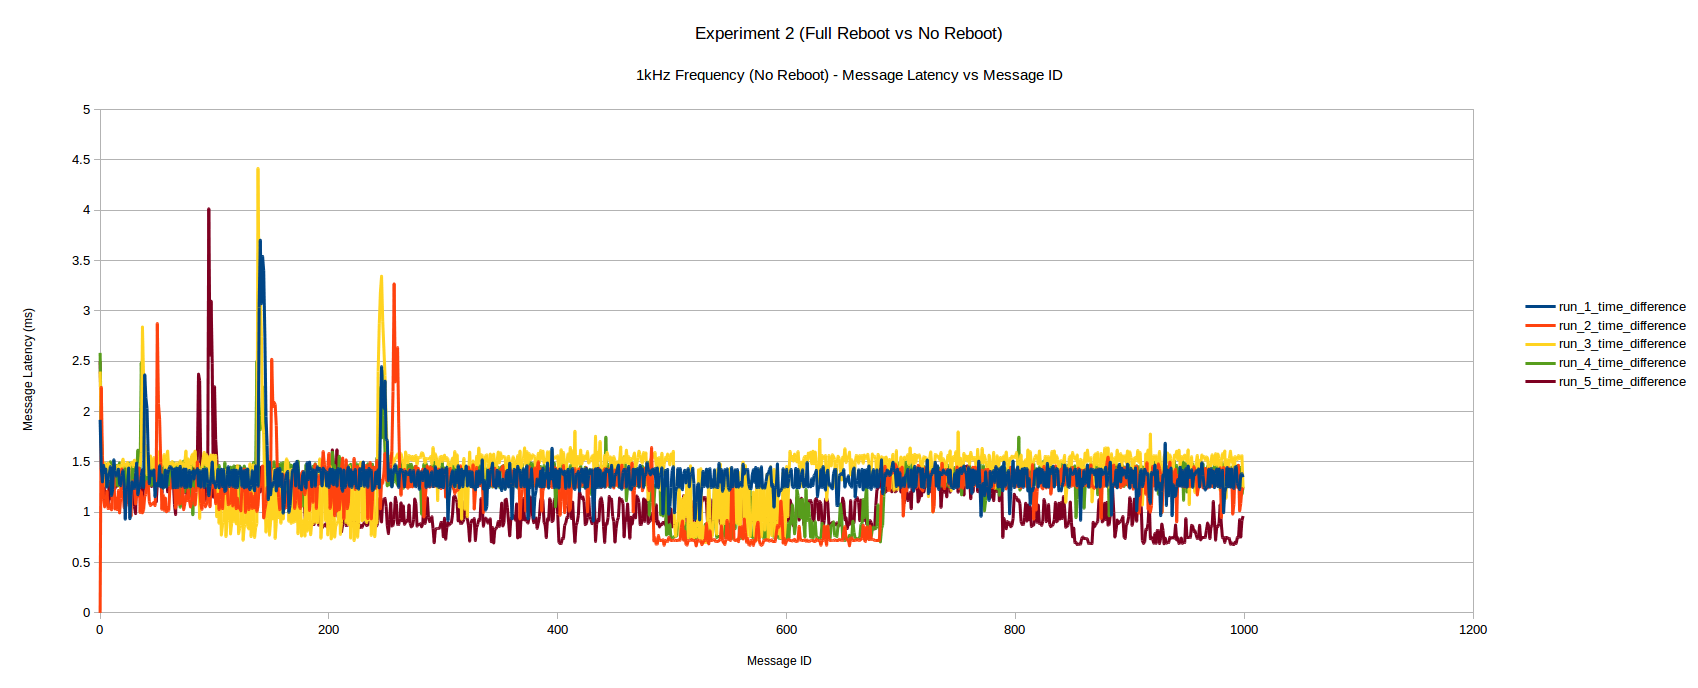
\includegraphics[width=\textwidth]{images/no-reboot-1khz.png}
\caption{Experiment 2 - No Reboot 1KHz Message Frequency}
\label{exp2-fullreboot-1khz}
\end{figure}

\begin{figure}
\centering
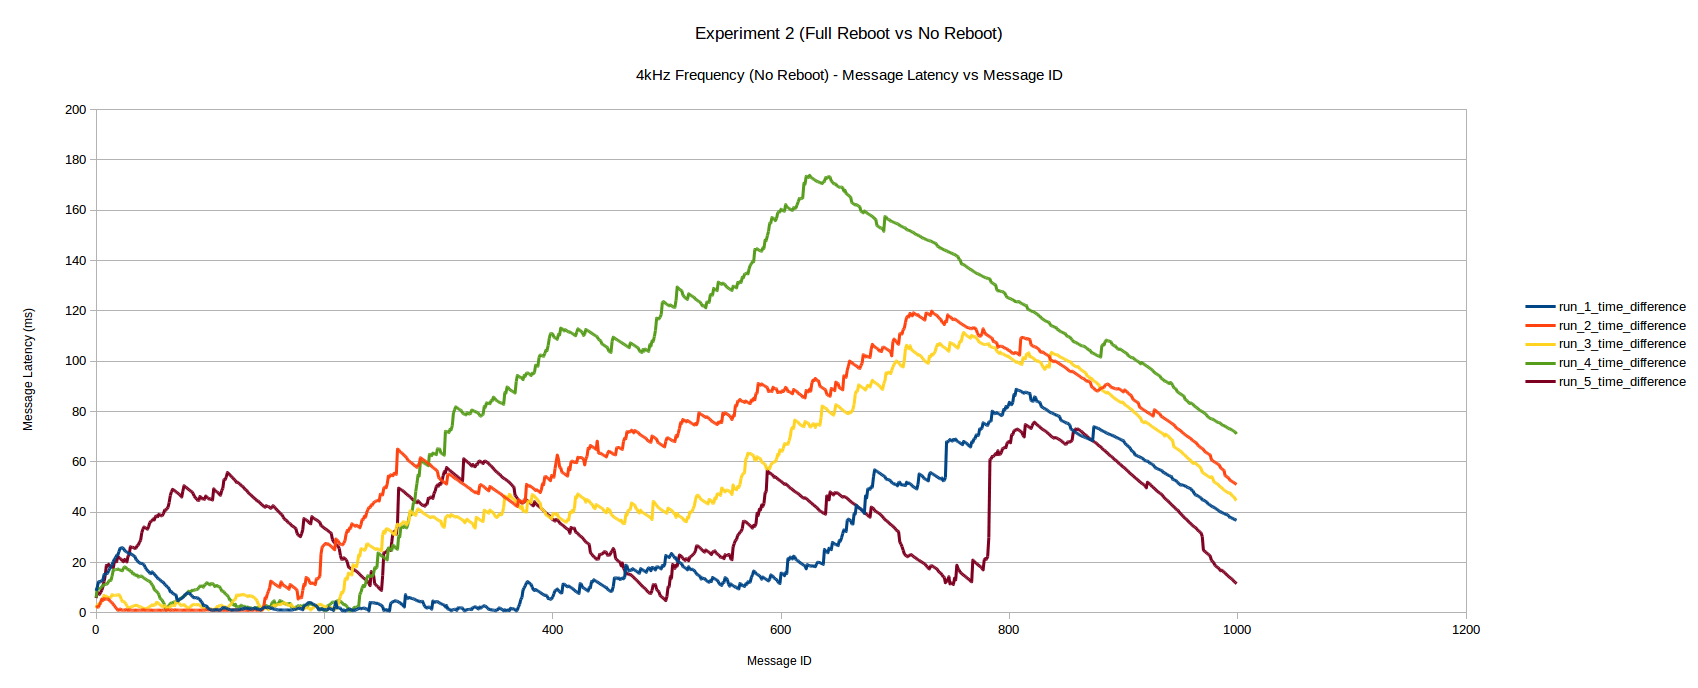
\includegraphics[width=\textwidth]{images/no-reboot-4khz.png}
\caption{Experiment 2 - No Reboot 4KHz Message Frequency}
\label{exp2-noreboot-4khz}
\end{figure}

\begin{figure}
\centering
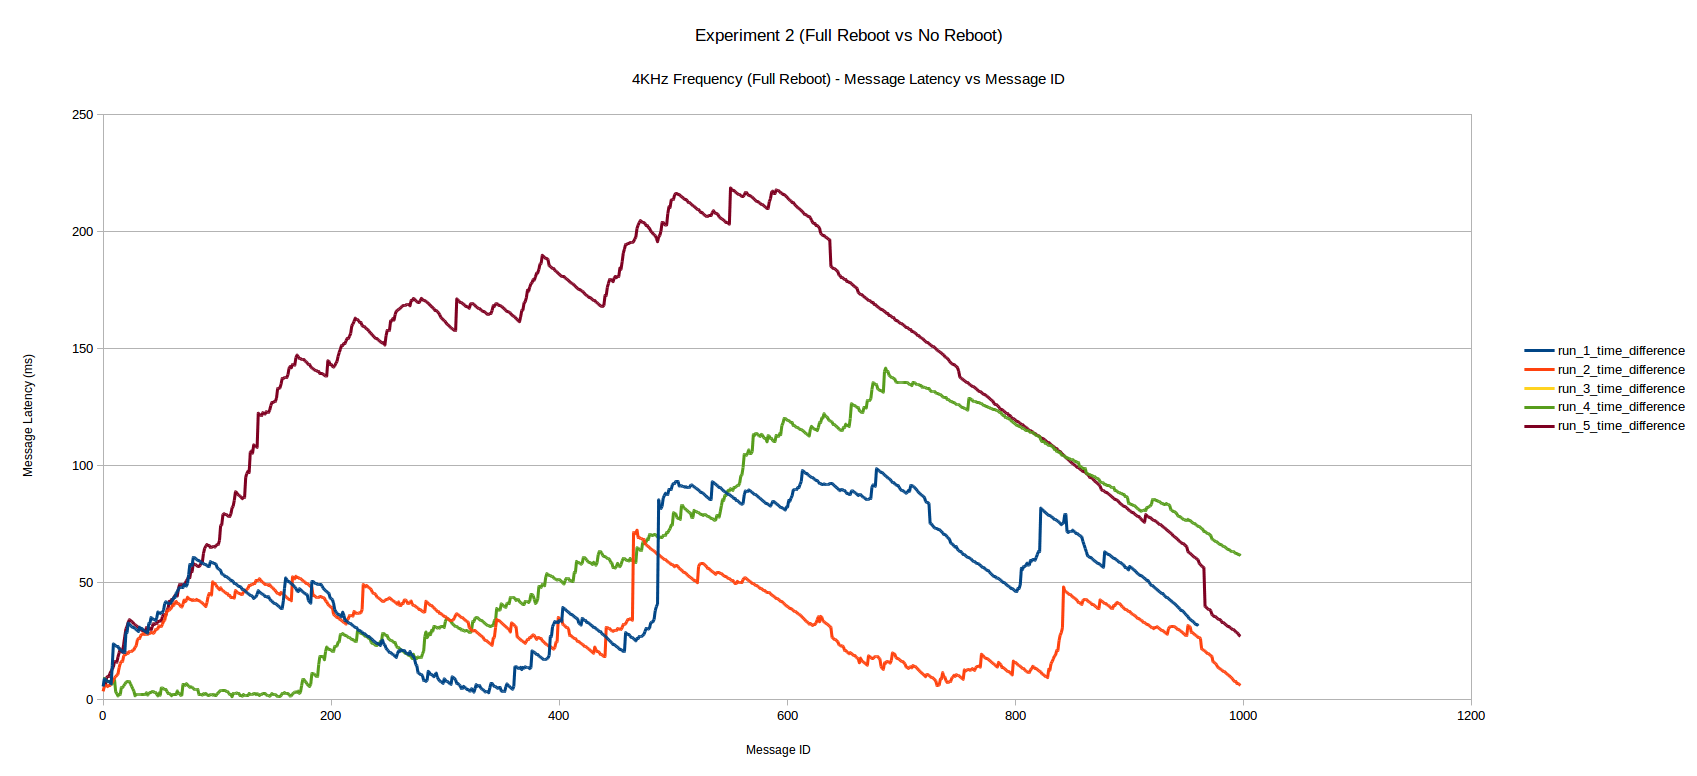
\includegraphics[width=\textwidth]{images/full-reboot-4khz.png}
\caption{Experiment 2 - Full Reboot 4KHz Message Frequency}
\label{exp2-fullreboot-4khz}
\end{figure}

\begin{figure}
\centering
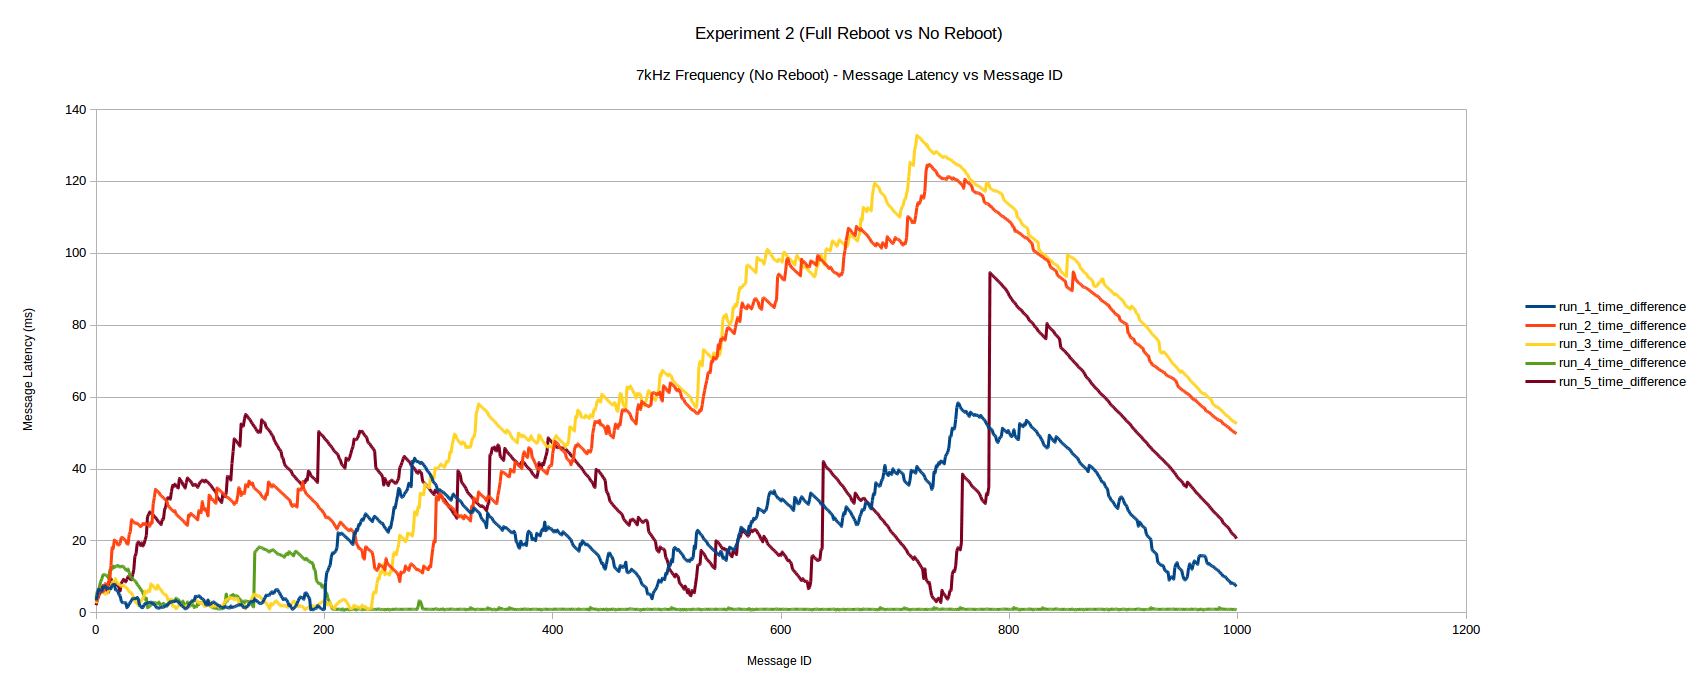
\includegraphics[width=\textwidth]{images/no-reboot-7khz.png}
\caption{Experiment 2 - No Reboot 7KHz Message Frequency}
\label{exp2-noreboot-7khz}
\end{figure}

\begin{figure}
\centering
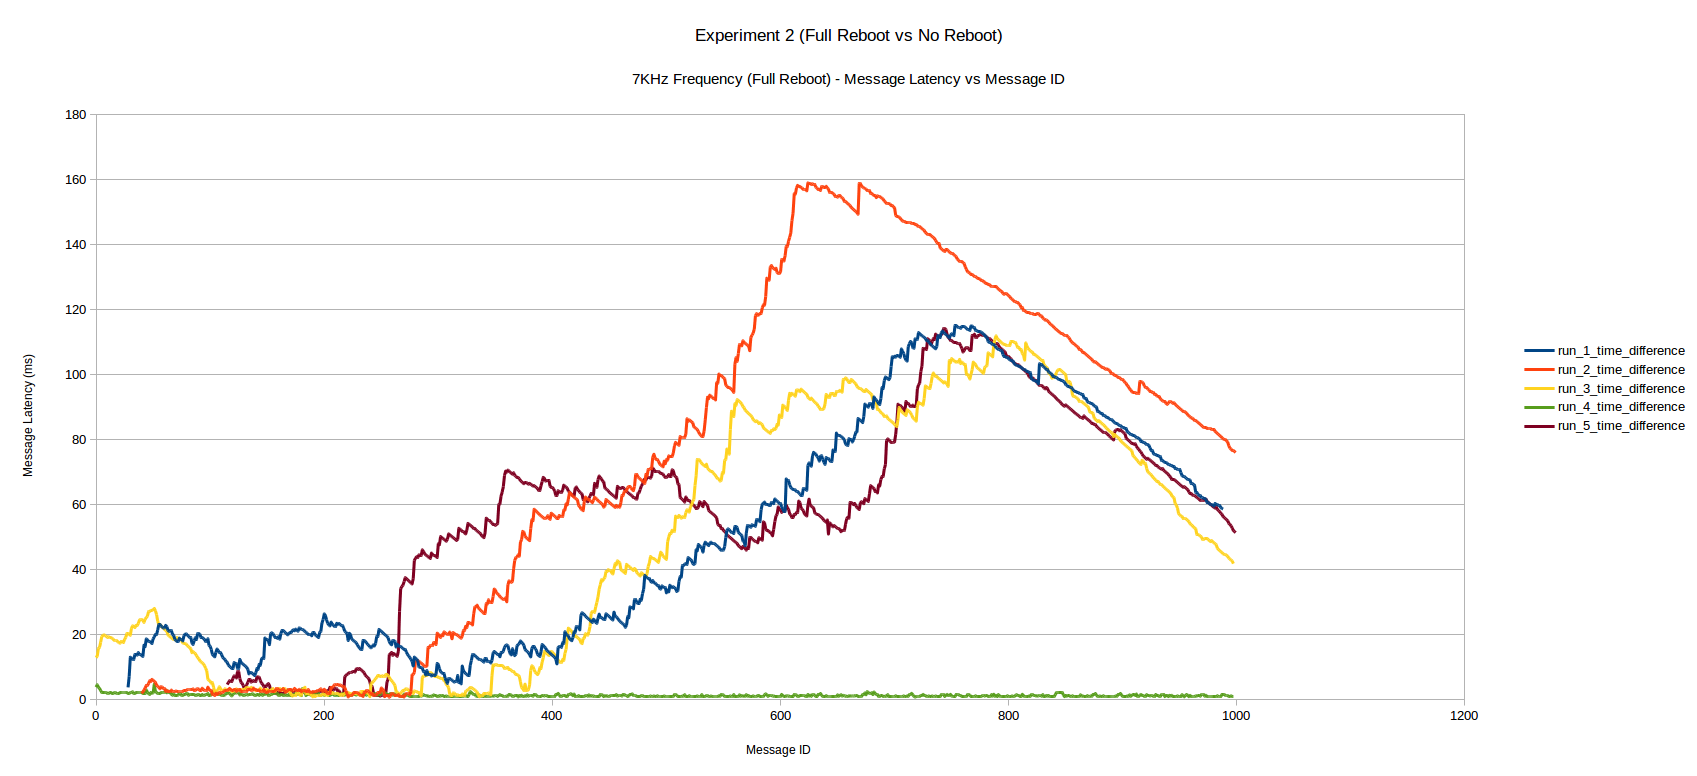
\includegraphics[width=\textwidth]{images/full-reboot-7khz.png}
\caption{Experiment 2 - Full Reboot 7KHz Message Frequency}
\label{exp2-fullreboot-7khz}
\end{figure}

\begin{figure}
\centering
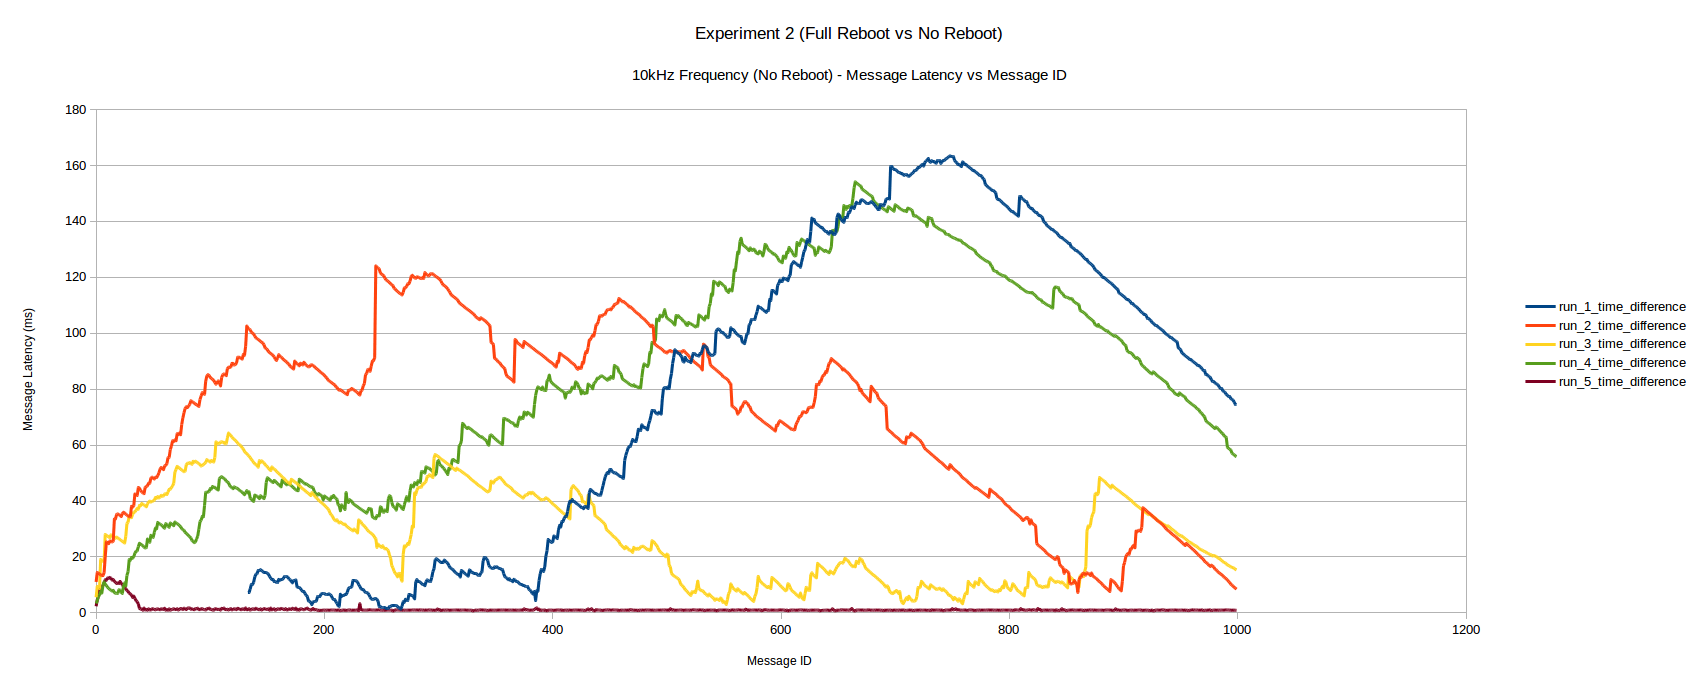
\includegraphics[width=\textwidth]{images/no-reboot-10khz.png}
\caption{Experiment 2 - No Reboot 10KHz Message Frequency}
\label{exp2-noreboot-10khz}
\end{figure}

\begin{figure}
\centering
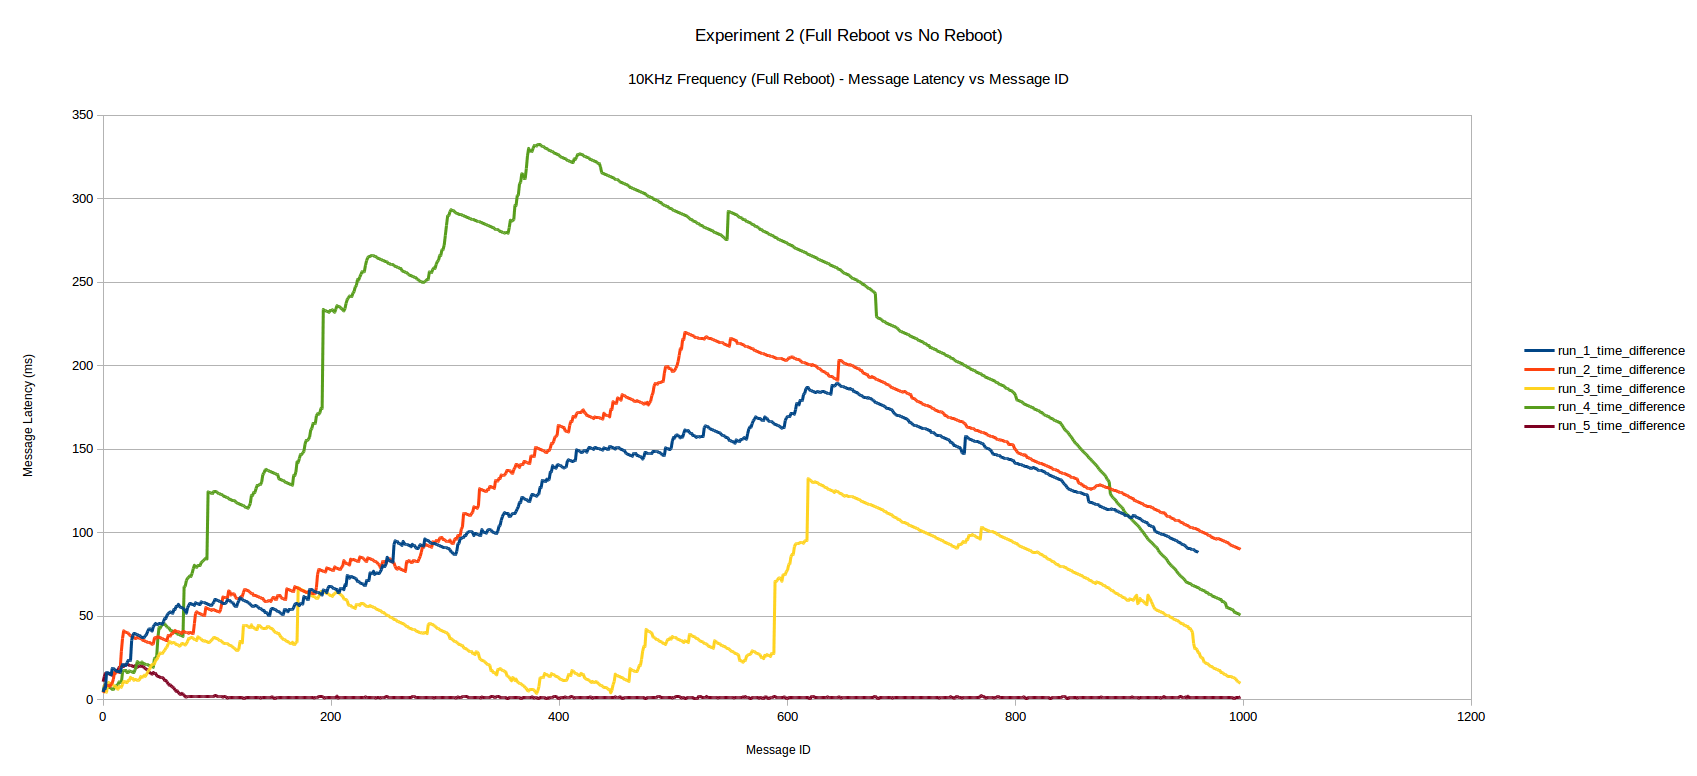
\includegraphics[width=\textwidth]{images/full-reboot-10khz.png}
\caption{Experiment 2 - Full Reboot 10KHz Message Frequency}
\label{exp2-fullreboot-10khz}
\end{figure}

\chapter{Code}

\section{Experiment 1 - Initial Code}
\label{Exp1InitCode}

\subsection{Sender and Receiver}

\begin{lstlisting}[language=Python]
#!/usr/bin/env python

import rospy
from rosberry_experiments.msg import StampedMessage
import time
import sys

N = None
RATE = None
f = None

def listener(msg):
    recv_time = rospy.get_rostime()
    send_time = msg.t

    f.write(str(msg.id))
    f.write(",")
    f.write(str(send_time))
    f.write(",")
    f.write(str(recv_time))
    f.write("\n")

def talker():
    pub = rospy.Publisher('chatter_m', StampedMessage, queue_size=RATE)
    rospy.init_node('talker', anonymous=True)
    rate = rospy.Rate(RATE)
    for i in xrange(N):
        hello_str = "hello world"
        timestamp = rospy.get_rostime()
        pub.publish(id=i, t=timestamp ,message=hello_str )
        rate.sleep()

def main():
    global RATE, N, f
    RATE = int(sys.argv[1])
    N = int(sys.argv[2])
    f = open("times_"+str(RATE)+".txt", "w+")
    print RATE, N
    try:
        sub = rospy.Subscriber("chatter_s", StampedMessage, listener)
        talker()
        rospy.sleep(5)
        f.close()
    except rospy.ROSInterruptException:
        pass


if __name__ == '__main__':
    main()
\end{lstlisting}

\subsection{Echoer}
\begin{lstlisting}[language=Python]
#!/usr/bin/env python

import rospy
from rosberry_experiments.msg import StampedMessage
import time
import sys

RATE = None

def listener(msg, args):
    rate = rospy.Rate(RATE)
    pub = args[0]
    pub.publish(msg)
    rate.sleep()

def main():
    global RATE
    RATE = int(sys.argv[1])
    try:
        rospy.init_node('talker1', anonymous=True)
        pub = rospy.Publisher('chatter_s', StampedMessage, queue_size=RATE)
        sub = rospy.Subscriber("chatter_m", StampedMessage, listener, callback_args=[pub])
        rospy.spin()
    except rospy.ROSInterruptException:
        pass

if __name__ == '__main__':
    main()
\end{lstlisting}

\section{Experiment 1 - Revised Code}

\subsection{Sender and Receiver}
\begin{lstlisting}[language=Python]
#!/usr/bin/env python

import rospy
from rosberry_experiments.msg import StampedMessage
import time
import sys

N = None
RATE = None
f = None

def listener(msg):
    recv_time = rospy.get_rostime()
    sent_time = msg.t
    f.write(str(msg.id) + "," + str(sent_time) + "," + str(recv_time) + "\n")

def talker():
    pub = rospy.Publisher('chatter_m', StampedMessage, queue_size=N)
    rospy.init_node('talker', anonymous=True)
    rate = rospy.Rate(RATE)
    for i in xrange(N):
        hello_str = "hello world"
        timestamp = rospy.get_rostime()
        pub.publish(id=i, t=timestamp, message=hello_str )

        rate.sleep()

def main():
    global RATE, N, f
    RATE = int(sys.argv[1])
    N = int(sys.argv[2])
    f = open("times_"+str(RATE)+".txt", "w+")
    print RATE, N
    try:
        sub = rospy.Subscriber("chatter_s", StampedMessage, listener)
        talker()
        rospy.sleep(5)
        f.close()

    except rospy.ROSInterruptException:
        print "Exception: ROSInterruptException"


if __name__ == '__main__':
    main()
\end{lstlisting}

\subsection{Echoer}
\begin{lstlisting}[language=Python]
#!/usr/bin/env python

import rospy
from rosberry_experiments.msg import StampedMessage
import time
import sys

def listener(msg, args):
    pub = args[0]
    pub.publish(msg)

def main():
    N = int(sys.argv[2])
    rospy.init_node('talker1', anonymous=True)
    pub = rospy.Publisher('chatter_s',
						StampedMessage, queue_size=N)

    sub = rospy.Subscriber("chatter_m",
						StampedMessage, listener, callback_args=[pub])
    try:
        rospy.spin()
    except rospy.ROSInterruptException:
        print "Exception: ROSInterruptException"

if __name__ == '__main__':
    main()
\end{lstlisting}

\chapter{Running the Programs}

To compile this dissertation:
\begin{verbatim}

	> pdflatex dissertation
	> bibtex dissertation
	> pdflatex dissertation
    > pdflatex dissertation

\end{verbatim}


An example of running from the command line is as follows:
\begin{verbatim}
	> rosrun rosberry_experiments run_experiment.py
\end{verbatim}


\chapter{Generating Random Graphs (Example Appendix)}
\label{sec:randomGraph}

\begin{verbatim}
	> java RandomGraph 100 0.9 > 100-90-00.clq
\end{verbatim}
\end{appendices}

%%%%%%%%%%%%%%%%%%%%
%   BIBLIOGRAPHY   %
%%%%%%%%%%%%%%%%%%%%

\bibliographystyle{plain}
\bibliography{bib}

\end{document}
